\begin{tikzpicture}[scale=.2, anchor=south west]
\node[draw=black, rectangle split, rectangle split parts=2] (sn0x8def9a0W-4) at (-4.75, -12) {
\begin{tikzpicture}[scale=.2]
\node[circle, scale=0.75, fill] (tid0) at (3.75,0){};
\node[circle, scale=0.75, fill] (tid1) at (1.5,1.5){};
\node[circle, scale=0.75, fill] (tid3) at (1.5,3){};
\node[circle, scale=0.75, fill] (tid7) at (0.75,4.5){};
\node[circle, scale=0.75, fill, red] (tid10) at (0.75,6){};
\draw[](tid7) -- (tid10);
\node[circle, scale=0.75, fill, red] (tid8) at (2.25,4.5){};
\draw[](tid3) -- (tid7);
\draw[](tid3) -- (tid8);
\draw[](tid1) -- (tid3);
\node[circle, scale=0.75, fill] (tid2) at (5.25,1.5){};
\node[circle, scale=0.75, fill] (tid4) at (3.75,3){};
\node[circle, scale=0.75, fill] (tid9) at (3.75,4.5){};
\draw[](tid4) -- (tid9);
\node[circle, scale=0.75, fill] (tid5) at (5.25,3){};
\node[circle, scale=0.75, fill] (tid6) at (6.75,3){};
\draw[](tid2) -- (tid4);
\draw[](tid2) -- (tid5);
\draw[](tid2) -- (tid6);
\draw[](tid0) -- (tid1);
\draw[](tid0) -- (tid2);

\end{tikzpicture}
\nodepart{two}
\footnotesize{6.82812}
};
\node[draw=black, rectangle split, rectangle split parts=2] (sn0x8df10a8W-13) at (-13.5, -24) {
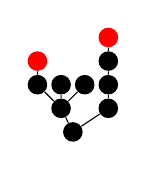
\begin{tikzpicture}[scale=.2]
\node[circle, scale=0.75, fill] (tid0) at (3,0){};
\node[circle, scale=0.75, fill] (tid1) at (2.25,1.5){};
\node[circle, scale=0.75, fill] (tid4) at (0.75,3){};
\node[circle, scale=0.75, fill, red] (tid8) at (0.75,4.5){};
\draw[](tid4) -- (tid8);
\node[circle, scale=0.75, fill] (tid5) at (2.25,3){};
\node[circle, scale=0.75, fill] (tid6) at (3.75,3){};
\draw[](tid1) -- (tid4);
\draw[](tid1) -- (tid5);
\draw[](tid1) -- (tid6);
\node[circle, scale=0.75, fill] (tid2) at (5.25,1.5){};
\node[circle, scale=0.75, fill] (tid3) at (5.25,3){};
\node[circle, scale=0.75, fill] (tid7) at (5.25,4.5){};
\node[circle, scale=0.75, fill, red] (tid9) at (5.25,6){};
\draw[](tid7) -- (tid9);
\draw[](tid3) -- (tid7);
\draw[](tid2) -- (tid3);
\draw[](tid0) -- (tid1);
\draw[](tid0) -- (tid2);

\end{tikzpicture}
\nodepart{two}
\footnotesize{6.35938}
};
\node[draw=black, rectangle split, rectangle split parts=2] (sn0x8df1010W-12) at (-12.75, -36) {
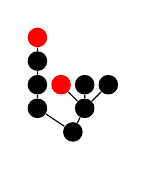
\begin{tikzpicture}[scale=.2]
\node[circle, scale=0.75, fill] (tid0) at (3,0){};
\node[circle, scale=0.75, fill] (tid1) at (0.75,1.5){};
\node[circle, scale=0.75, fill] (tid3) at (0.75,3){};
\node[circle, scale=0.75, fill] (tid7) at (0.75,4.5){};
\node[circle, scale=0.75, fill, red] (tid8) at (0.75,6){};
\draw[](tid7) -- (tid8);
\draw[](tid3) -- (tid7);
\draw[](tid1) -- (tid3);
\node[circle, scale=0.75, fill] (tid2) at (3.75,1.5){};
\node[circle, scale=0.75, fill, red] (tid4) at (2.25,3){};
\node[circle, scale=0.75, fill] (tid5) at (3.75,3){};
\node[circle, scale=0.75, fill] (tid6) at (5.25,3){};
\draw[](tid2) -- (tid4);
\draw[](tid2) -- (tid5);
\draw[](tid2) -- (tid6);
\draw[](tid0) -- (tid1);
\draw[](tid0) -- (tid2);

\end{tikzpicture}
\nodepart{two}
\footnotesize{5.92188}
};
\node[draw=black, rectangle split, rectangle split parts=2] (sn0x8df17c0W-15) at (-15.25, -48) {
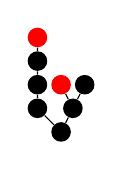
\begin{tikzpicture}[scale=.2]
\node[circle, scale=0.75, fill] (tid0) at (2.25,0){};
\node[circle, scale=0.75, fill] (tid1) at (0.75,1.5){};
\node[circle, scale=0.75, fill] (tid3) at (0.75,3){};
\node[circle, scale=0.75, fill] (tid6) at (0.75,4.5){};
\node[circle, scale=0.75, fill, red] (tid7) at (0.75,6){};
\draw[](tid6) -- (tid7);
\draw[](tid3) -- (tid6);
\draw[](tid1) -- (tid3);
\node[circle, scale=0.75, fill] (tid2) at (3,1.5){};
\node[circle, scale=0.75, fill, red] (tid4) at (2.25,3){};
\node[circle, scale=0.75, fill] (tid5) at (3.75,3){};
\draw[](tid2) -- (tid4);
\draw[](tid2) -- (tid5);
\draw[](tid0) -- (tid1);
\draw[](tid0) -- (tid2);

\end{tikzpicture}
\nodepart{two}
\footnotesize{5.54688}
};
\node[draw=black, rectangle split, rectangle split parts=2] (sn0x8df2260W-24) at (-24.25, -60) {
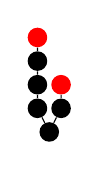
\begin{tikzpicture}[scale=.2]
\node[circle, scale=0.75, fill] (tid0) at (1.5,0){};
\node[circle, scale=0.75, fill] (tid1) at (0.75,1.5){};
\node[circle, scale=0.75, fill] (tid3) at (0.75,3){};
\node[circle, scale=0.75, fill] (tid5) at (0.75,4.5){};
\node[circle, scale=0.75, fill, red] (tid6) at (0.75,6){};
\draw[](tid5) -- (tid6);
\draw[](tid3) -- (tid5);
\draw[](tid1) -- (tid3);
\node[circle, scale=0.75, fill] (tid2) at (2.25,1.5){};
\node[circle, scale=0.75, fill, red] (tid4) at (2.25,3){};
\draw[](tid2) -- (tid4);
\draw[](tid0) -- (tid1);
\draw[](tid0) -- (tid2);

\end{tikzpicture}
\nodepart{two}
\footnotesize{5.25}
};
\node[draw=black, rectangle split, rectangle split parts=2] (sn0x8df2658W-18) at (-18.75, -72) {
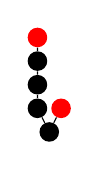
\begin{tikzpicture}[scale=.2]
\node[circle, scale=0.75, fill] (tid0) at (1.5,0){};
\node[circle, scale=0.75, fill] (tid1) at (0.75,1.5){};
\node[circle, scale=0.75, fill] (tid3) at (0.75,3){};
\node[circle, scale=0.75, fill] (tid4) at (0.75,4.5){};
\node[circle, scale=0.75, fill, red] (tid5) at (0.75,6){};
\draw[](tid4) -- (tid5);
\draw[](tid3) -- (tid4);
\draw[](tid1) -- (tid3);
\node[circle, scale=0.75, fill, red] (tid2) at (2.25,1.5){};
\draw[](tid0) -- (tid1);
\draw[](tid0) -- (tid2);

\end{tikzpicture}
\nodepart{two}
\footnotesize{5.0625}
};
\node[draw=black, rectangle split, rectangle split parts=2] (sn0x8df2c20W-10) at (-10, -84) {
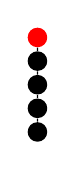
\begin{tikzpicture}[scale=.2]
\node[circle, scale=0.75, fill] (tid0) at (0.75,0){};
\node[circle, scale=0.75, fill] (tid1) at (0.75,1.5){};
\node[circle, scale=0.75, fill] (tid2) at (0.75,3){};
\node[circle, scale=0.75, fill] (tid3) at (0.75,4.5){};
\node[circle, scale=0.75, fill, red] (tid4) at (0.75,6){};
\draw[](tid3) -- (tid4);
\draw[](tid2) -- (tid3);
\draw[](tid1) -- (tid2);
\draw[](tid0) -- (tid1);

\end{tikzpicture}
\nodepart{two}
\footnotesize{5}
};
\node[draw=black, rectangle split, rectangle split parts=2] (sn0x8df2f28W-4) at (-4.25, -96) {
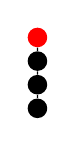
\begin{tikzpicture}[scale=.2]
\node[circle, scale=0.75, fill] (tid0) at (0.75,0){};
\node[circle, scale=0.75, fill] (tid1) at (0.75,1.5){};
\node[circle, scale=0.75, fill] (tid2) at (0.75,3){};
\node[circle, scale=0.75, fill, red] (tid3) at (0.75,4.5){};
\draw[](tid2) -- (tid3);
\draw[](tid1) -- (tid2);
\draw[](tid0) -- (tid1);

\end{tikzpicture}
\nodepart{two}
\footnotesize{4}
};
\node[draw=black, rectangle split, rectangle split parts=2] (sn0x8df2fc0W-4) at (-4.25, -108) {
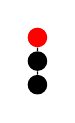
\begin{tikzpicture}[scale=.2]
\node[circle, scale=0.75, fill] (tid0) at (0.75,0){};
\node[circle, scale=0.75, fill] (tid1) at (0.75,1.5){};
\node[circle, scale=0.75, fill, red] (tid2) at (0.75,3){};
\draw[](tid1) -- (tid2);
\draw[](tid0) -- (tid1);

\end{tikzpicture}
\nodepart{two}
\footnotesize{3}
};
\node[draw=black, rectangle split, rectangle split parts=2] (sn0x8df30c0W-1) at (-1.75, -120) {

\begin{tikzpicture}[scale=.2]
\node[circle, scale=0.75, fill] (tid0) at (0.75,0){};
\node[circle, scale=0.75, fill, red] (tid1) at (0.75,1.5){};
\draw[](tid0) -- (tid1);

\end{tikzpicture}
\nodepart{two}
\footnotesize{2}
};
\draw (sn0x8df2fc0W-4.south) -- (sn0x8df30c0W-1.north);
\draw (sn0x8df2f28W-4.south) -- (sn0x8df2fc0W-4.north);
\draw (sn0x8df2c20W-10.south) -- (sn0x8df2f28W-4.north);
\node[draw=black, rectangle split, rectangle split parts=2] (sn0x8df2d88W-6) at (-6.5, -84) {
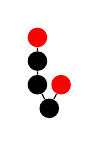
\begin{tikzpicture}[scale=.2]
\node[circle, scale=0.75, fill] (tid0) at (1.5,0){};
\node[circle, scale=0.75, fill] (tid1) at (0.75,1.5){};
\node[circle, scale=0.75, fill] (tid3) at (0.75,3){};
\node[circle, scale=0.75, fill, red] (tid4) at (0.75,4.5){};
\draw[](tid3) -- (tid4);
\draw[](tid1) -- (tid3);
\node[circle, scale=0.75, fill, red] (tid2) at (2.25,1.5){};
\draw[](tid0) -- (tid1);
\draw[](tid0) -- (tid2);

\end{tikzpicture}
\nodepart{two}
\footnotesize{4.125}
};
\node[draw=black, rectangle split, rectangle split parts=2] (sn0x8df3410W0) at (-0.75, -96) {
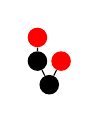
\begin{tikzpicture}[scale=.2]
\node[circle, scale=0.75, fill] (tid0) at (1.5,0){};
\node[circle, scale=0.75, fill] (tid1) at (0.75,1.5){};
\node[circle, scale=0.75, fill, red] (tid3) at (0.75,3){};
\draw[](tid1) -- (tid3);
\node[circle, scale=0.75, fill, red] (tid2) at (2.25,1.5){};
\draw[](tid0) -- (tid1);
\draw[](tid0) -- (tid2);

\end{tikzpicture}
\nodepart{two}
\footnotesize{3.25}
};
\node[draw=black, rectangle split, rectangle split parts=2] (sn0x8df3608W0) at (-0.75, -108) {

\begin{tikzpicture}[scale=.2]
\node[circle, scale=0.75, fill] (tid0) at (1.5,0){};
\node[circle, scale=0.75, fill, red] (tid1) at (0.75,1.5){};
\node[circle, scale=0.75, fill, red] (tid2) at (2.25,1.5){};
\draw[](tid0) -- (tid1);
\draw[](tid0) -- (tid2);

\end{tikzpicture}
\nodepart{two}
\footnotesize{2.5}
};
\draw (sn0x8df3608W0.south) -- (sn0x8df30c0W-1.north);
\draw (sn0x8df3410W0.south) -- (sn0x8df2fc0W-4.north);
\draw (sn0x8df3410W0.south) -- (sn0x8df3608W0.north);
\draw (sn0x8df2d88W-6.south) -- (sn0x8df2f28W-4.north);
\draw (sn0x8df2d88W-6.south) -- (sn0x8df3410W0.north);
\draw (sn0x8df2658W-18.south) -- (sn0x8df2c20W-10.north);
\draw (sn0x8df2658W-18.south) -- (sn0x8df2d88W-6.north);
\node[draw=black, rectangle split, rectangle split parts=2] (sn0x8df2a00W-13) at (-13.75, -72) {
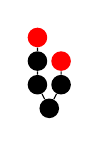
\begin{tikzpicture}[scale=.2]
\node[circle, scale=0.75, fill] (tid0) at (1.5,0){};
\node[circle, scale=0.75, fill] (tid1) at (0.75,1.5){};
\node[circle, scale=0.75, fill] (tid3) at (0.75,3){};
\node[circle, scale=0.75, fill, red] (tid5) at (0.75,4.5){};
\draw[](tid3) -- (tid5);
\draw[](tid1) -- (tid3);
\node[circle, scale=0.75, fill] (tid2) at (2.25,1.5){};
\node[circle, scale=0.75, fill, red] (tid4) at (2.25,3){};
\draw[](tid2) -- (tid4);
\draw[](tid0) -- (tid1);
\draw[](tid0) -- (tid2);

\end{tikzpicture}
\nodepart{two}
\footnotesize{4.4375}
};
\node[draw=black, rectangle split, rectangle split parts=2] (sn0x8df3570W-1) at (-1.5, -84) {
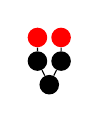
\begin{tikzpicture}[scale=.2]
\node[circle, scale=0.75, fill] (tid0) at (1.5,0){};
\node[circle, scale=0.75, fill] (tid1) at (0.75,1.5){};
\node[circle, scale=0.75, fill, red] (tid3) at (0.75,3){};
\draw[](tid1) -- (tid3);
\node[circle, scale=0.75, fill] (tid2) at (2.25,1.5){};
\node[circle, scale=0.75, fill, red] (tid4) at (2.25,3){};
\draw[](tid2) -- (tid4);
\draw[](tid0) -- (tid1);
\draw[](tid0) -- (tid2);

\end{tikzpicture}
\nodepart{two}
\footnotesize{3.75}
};
\draw (sn0x8df3570W-1.south) -- (sn0x8df3410W0.north);
\draw (sn0x8df2a00W-13.south) -- (sn0x8df2d88W-6.north);
\draw (sn0x8df2a00W-13.south) -- (sn0x8df3570W-1.north);
\draw (sn0x8df2260W-24.south) -- (sn0x8df2658W-18.north);
\draw (sn0x8df2260W-24.south) -- (sn0x8df2a00W-13.north);
\node[draw=black, rectangle split, rectangle split parts=2] (sn0x8df2070W-19) at (-19.25, -60) {
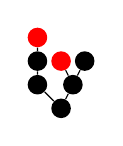
\begin{tikzpicture}[scale=.2]
\node[circle, scale=0.75, fill] (tid0) at (2.25,0){};
\node[circle, scale=0.75, fill] (tid1) at (0.75,1.5){};
\node[circle, scale=0.75, fill] (tid3) at (0.75,3){};
\node[circle, scale=0.75, fill, red] (tid6) at (0.75,4.5){};
\draw[](tid3) -- (tid6);
\draw[](tid1) -- (tid3);
\node[circle, scale=0.75, fill] (tid2) at (3,1.5){};
\node[circle, scale=0.75, fill, red] (tid4) at (2.25,3){};
\node[circle, scale=0.75, fill] (tid5) at (3.75,3){};
\draw[](tid2) -- (tid4);
\draw[](tid2) -- (tid5);
\draw[](tid0) -- (tid1);
\draw[](tid0) -- (tid2);

\end{tikzpicture}
\nodepart{two}
\footnotesize{4.84375}
};
\node[draw=black, rectangle split, rectangle split parts=2] (sn0x8df3ca8W-8) at (-8.75, -72) {
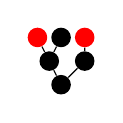
\begin{tikzpicture}[scale=.2]
\node[circle, scale=0.75, fill] (tid0) at (2.25,0){};
\node[circle, scale=0.75, fill] (tid1) at (1.5,1.5){};
\node[circle, scale=0.75, fill, red] (tid3) at (0.75,3){};
\node[circle, scale=0.75, fill] (tid4) at (2.25,3){};
\draw[](tid1) -- (tid3);
\draw[](tid1) -- (tid4);
\node[circle, scale=0.75, fill] (tid2) at (3.75,1.5){};
\node[circle, scale=0.75, fill, red] (tid5) at (3.75,3){};
\draw[](tid2) -- (tid5);
\draw[](tid0) -- (tid1);
\draw[](tid0) -- (tid2);

\end{tikzpicture}
\nodepart{two}
\footnotesize{4.25}
};
\node[draw=black, rectangle split, rectangle split parts=2] (sn0x8df4250W3) at (3.5, -84) {
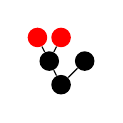
\begin{tikzpicture}[scale=.2]
\node[circle, scale=0.75, fill] (tid0) at (2.25,0){};
\node[circle, scale=0.75, fill] (tid1) at (1.5,1.5){};
\node[circle, scale=0.75, fill, red] (tid3) at (0.75,3){};
\node[circle, scale=0.75, fill, red] (tid4) at (2.25,3){};
\draw[](tid1) -- (tid3);
\draw[](tid1) -- (tid4);
\node[circle, scale=0.75, fill] (tid2) at (3.75,1.5){};
\draw[](tid0) -- (tid1);
\draw[](tid0) -- (tid2);

\end{tikzpicture}
\nodepart{two}
\footnotesize{3.75}
};
\draw (sn0x8df4250W3.south) -- (sn0x8df3410W0.north);
\draw (sn0x8df3ca8W-8.south) -- (sn0x8df3570W-1.north);
\draw (sn0x8df3ca8W-8.south) -- (sn0x8df4250W3.north);
\node[draw=black, rectangle split, rectangle split parts=2] (sn0x8df3d10W-2) at (-2.25, -72) {
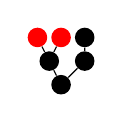
\begin{tikzpicture}[scale=.2]
\node[circle, scale=0.75, fill] (tid0) at (2.25,0){};
\node[circle, scale=0.75, fill] (tid1) at (1.5,1.5){};
\node[circle, scale=0.75, fill, red] (tid3) at (0.75,3){};
\node[circle, scale=0.75, fill, red] (tid4) at (2.25,3){};
\draw[](tid1) -- (tid3);
\draw[](tid1) -- (tid4);
\node[circle, scale=0.75, fill] (tid2) at (3.75,1.5){};
\node[circle, scale=0.75, fill] (tid5) at (3.75,3){};
\draw[](tid2) -- (tid5);
\draw[](tid0) -- (tid1);
\draw[](tid0) -- (tid2);

\end{tikzpicture}
\nodepart{two}
\footnotesize{4.25}
};
\draw (sn0x8df3d10W-2.south) -- (sn0x8df3570W-1.north);
\draw (sn0x8df2070W-19.south) -- (sn0x8df2a00W-13.north);
\draw (sn0x8df2070W-19.south) -- (sn0x8df3ca8W-8.north);
\draw (sn0x8df2070W-19.south) -- (sn0x8df3d10W-2.north);
\draw (sn0x8df17c0W-15.south) -- (sn0x8df2260W-24.north);
\draw (sn0x8df17c0W-15.south) -- (sn0x8df2070W-19.north);
\node[draw=black, rectangle split, rectangle split parts=2] (sn0x8df1ec8W-8) at (-8.75, -48) {
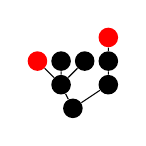
\begin{tikzpicture}[scale=.2]
\node[circle, scale=0.75, fill] (tid0) at (3,0){};
\node[circle, scale=0.75, fill] (tid1) at (2.25,1.5){};
\node[circle, scale=0.75, fill, red] (tid4) at (0.75,3){};
\node[circle, scale=0.75, fill] (tid5) at (2.25,3){};
\node[circle, scale=0.75, fill] (tid6) at (3.75,3){};
\draw[](tid1) -- (tid4);
\draw[](tid1) -- (tid5);
\draw[](tid1) -- (tid6);
\node[circle, scale=0.75, fill] (tid2) at (5.25,1.5){};
\node[circle, scale=0.75, fill] (tid3) at (5.25,3){};
\node[circle, scale=0.75, fill, red] (tid7) at (5.25,4.5){};
\draw[](tid3) -- (tid7);
\draw[](tid2) -- (tid3);
\draw[](tid0) -- (tid1);
\draw[](tid0) -- (tid2);

\end{tikzpicture}
\nodepart{two}
\footnotesize{5.29688}
};
\node[draw=black, rectangle split, rectangle split parts=2] (sn0x8df44e0W-12) at (-12.75, -60) {
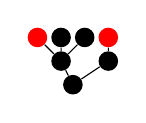
\begin{tikzpicture}[scale=.2]
\node[circle, scale=0.75, fill] (tid0) at (3,0){};
\node[circle, scale=0.75, fill] (tid1) at (2.25,1.5){};
\node[circle, scale=0.75, fill, red] (tid3) at (0.75,3){};
\node[circle, scale=0.75, fill] (tid4) at (2.25,3){};
\node[circle, scale=0.75, fill] (tid5) at (3.75,3){};
\draw[](tid1) -- (tid3);
\draw[](tid1) -- (tid4);
\draw[](tid1) -- (tid5);
\node[circle, scale=0.75, fill] (tid2) at (5.25,1.5){};
\node[circle, scale=0.75, fill, red] (tid6) at (5.25,3){};
\draw[](tid2) -- (tid6);
\draw[](tid0) -- (tid1);
\draw[](tid0) -- (tid2);

\end{tikzpicture}
\nodepart{two}
\footnotesize{4.75}
};
\node[draw=black, rectangle split, rectangle split parts=2] (sn0x8df4ab8W4) at (4.25, -72) {
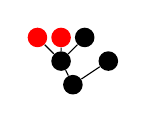
\begin{tikzpicture}[scale=.2]
\node[circle, scale=0.75, fill] (tid0) at (3,0){};
\node[circle, scale=0.75, fill] (tid1) at (2.25,1.5){};
\node[circle, scale=0.75, fill, red] (tid3) at (0.75,3){};
\node[circle, scale=0.75, fill, red] (tid4) at (2.25,3){};
\node[circle, scale=0.75, fill] (tid5) at (3.75,3){};
\draw[](tid1) -- (tid3);
\draw[](tid1) -- (tid4);
\draw[](tid1) -- (tid5);
\node[circle, scale=0.75, fill] (tid2) at (5.25,1.5){};
\draw[](tid0) -- (tid1);
\draw[](tid0) -- (tid2);

\end{tikzpicture}
\nodepart{two}
\footnotesize{4.25}
};
\draw (sn0x8df4ab8W4.south) -- (sn0x8df4250W3.north);
\draw (sn0x8df44e0W-12.south) -- (sn0x8df3ca8W-8.north);
\draw (sn0x8df44e0W-12.south) -- (sn0x8df4ab8W4.north);
\node[draw=black, rectangle split, rectangle split parts=2] (sn0x8df3ee0W-4) at (-4.75, -60) {
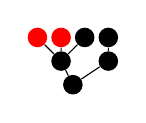
\begin{tikzpicture}[scale=.2]
\node[circle, scale=0.75, fill] (tid0) at (3,0){};
\node[circle, scale=0.75, fill] (tid1) at (2.25,1.5){};
\node[circle, scale=0.75, fill, red] (tid3) at (0.75,3){};
\node[circle, scale=0.75, fill, red] (tid4) at (2.25,3){};
\node[circle, scale=0.75, fill] (tid5) at (3.75,3){};
\draw[](tid1) -- (tid3);
\draw[](tid1) -- (tid4);
\draw[](tid1) -- (tid5);
\node[circle, scale=0.75, fill] (tid2) at (5.25,1.5){};
\node[circle, scale=0.75, fill] (tid6) at (5.25,3){};
\draw[](tid2) -- (tid6);
\draw[](tid0) -- (tid1);
\draw[](tid0) -- (tid2);

\end{tikzpicture}
\nodepart{two}
\footnotesize{4.75}
};
\draw (sn0x8df3ee0W-4.south) -- (sn0x8df3d10W-2.north);
\draw (sn0x8df3ee0W-4.south) -- (sn0x8df3ca8W-8.north);
\draw (sn0x8df1ec8W-8.south) -- (sn0x8df2070W-19.north);
\draw (sn0x8df1ec8W-8.south) -- (sn0x8df44e0W-12.north);
\draw (sn0x8df1ec8W-8.south) -- (sn0x8df3ee0W-4.north);
\draw (sn0x8df1010W-12.south) -- (sn0x8df17c0W-15.north);
\draw (sn0x8df1010W-12.south) -- (sn0x8df1ec8W-8.north);
\node[draw=black, rectangle split, rectangle split parts=2] (sn0x8df06c8W-4) at (-4.75, -36) {
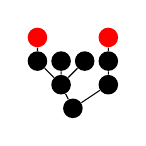
\begin{tikzpicture}[scale=.2]
\node[circle, scale=0.75, fill] (tid0) at (3,0){};
\node[circle, scale=0.75, fill] (tid1) at (2.25,1.5){};
\node[circle, scale=0.75, fill] (tid3) at (0.75,3){};
\node[circle, scale=0.75, fill, red] (tid8) at (0.75,4.5){};
\draw[](tid3) -- (tid8);
\node[circle, scale=0.75, fill] (tid5) at (2.25,3){};
\node[circle, scale=0.75, fill] (tid6) at (3.75,3){};
\draw[](tid1) -- (tid3);
\draw[](tid1) -- (tid5);
\draw[](tid1) -- (tid6);
\node[circle, scale=0.75, fill] (tid2) at (5.25,1.5){};
\node[circle, scale=0.75, fill] (tid4) at (5.25,3){};
\node[circle, scale=0.75, fill, red] (tid7) at (5.25,4.5){};
\draw[](tid4) -- (tid7);
\draw[](tid2) -- (tid4);
\draw[](tid0) -- (tid1);
\draw[](tid0) -- (tid2);

\end{tikzpicture}
\nodepart{two}
\footnotesize{5.79688}
};
\node[draw=black, rectangle split, rectangle split parts=2] (sn0x8df4bf8W0) at (-0.75, -48) {
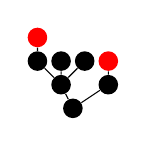
\begin{tikzpicture}[scale=.2]
\node[circle, scale=0.75, fill] (tid0) at (3,0){};
\node[circle, scale=0.75, fill] (tid1) at (2.25,1.5){};
\node[circle, scale=0.75, fill] (tid3) at (0.75,3){};
\node[circle, scale=0.75, fill, red] (tid7) at (0.75,4.5){};
\draw[](tid3) -- (tid7);
\node[circle, scale=0.75, fill] (tid4) at (2.25,3){};
\node[circle, scale=0.75, fill] (tid5) at (3.75,3){};
\draw[](tid1) -- (tid3);
\draw[](tid1) -- (tid4);
\draw[](tid1) -- (tid5);
\node[circle, scale=0.75, fill] (tid2) at (5.25,1.5){};
\node[circle, scale=0.75, fill, red] (tid6) at (5.25,3){};
\draw[](tid2) -- (tid6);
\draw[](tid0) -- (tid1);
\draw[](tid0) -- (tid2);

\end{tikzpicture}
\nodepart{two}
\footnotesize{5.29688}
};
\node[draw=black, rectangle split, rectangle split parts=2] (sn0x8df4dd0W3) at (3.25, -60) {
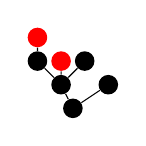
\begin{tikzpicture}[scale=.2]
\node[circle, scale=0.75, fill] (tid0) at (3,0){};
\node[circle, scale=0.75, fill] (tid1) at (2.25,1.5){};
\node[circle, scale=0.75, fill] (tid3) at (0.75,3){};
\node[circle, scale=0.75, fill, red] (tid6) at (0.75,4.5){};
\draw[](tid3) -- (tid6);
\node[circle, scale=0.75, fill, red] (tid4) at (2.25,3){};
\node[circle, scale=0.75, fill] (tid5) at (3.75,3){};
\draw[](tid1) -- (tid3);
\draw[](tid1) -- (tid4);
\draw[](tid1) -- (tid5);
\node[circle, scale=0.75, fill] (tid2) at (5.25,1.5){};
\draw[](tid0) -- (tid1);
\draw[](tid0) -- (tid2);

\end{tikzpicture}
\nodepart{two}
\footnotesize{4.84375}
};
\node[draw=black, rectangle split, rectangle split parts=2] (sn0x8df55d8W12) at (12.25, -72) {
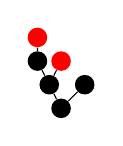
\begin{tikzpicture}[scale=.2]
\node[circle, scale=0.75, fill] (tid0) at (2.25,0){};
\node[circle, scale=0.75, fill] (tid1) at (1.5,1.5){};
\node[circle, scale=0.75, fill] (tid3) at (0.75,3){};
\node[circle, scale=0.75, fill, red] (tid5) at (0.75,4.5){};
\draw[](tid3) -- (tid5);
\node[circle, scale=0.75, fill, red] (tid4) at (2.25,3){};
\draw[](tid1) -- (tid3);
\draw[](tid1) -- (tid4);
\node[circle, scale=0.75, fill] (tid2) at (3.75,1.5){};
\draw[](tid0) -- (tid1);
\draw[](tid0) -- (tid2);

\end{tikzpicture}
\nodepart{two}
\footnotesize{4.4375}
};
\draw (sn0x8df55d8W12.south) -- (sn0x8df2d88W-6.north);
\draw (sn0x8df55d8W12.south) -- (sn0x8df4250W3.north);
\draw (sn0x8df4dd0W3.south) -- (sn0x8df55d8W12.north);
\draw (sn0x8df4dd0W3.south) -- (sn0x8df4ab8W4.north);
\draw (sn0x8df4bf8W0.south) -- (sn0x8df4dd0W3.north);
\draw (sn0x8df4bf8W0.south) -- (sn0x8df44e0W-12.north);
\node[draw=black, rectangle split, rectangle split parts=2] (sn0x8df5128W7) at (7.25, -48) {
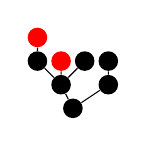
\begin{tikzpicture}[scale=.2]
\node[circle, scale=0.75, fill] (tid0) at (3,0){};
\node[circle, scale=0.75, fill] (tid1) at (2.25,1.5){};
\node[circle, scale=0.75, fill] (tid3) at (0.75,3){};
\node[circle, scale=0.75, fill, red] (tid7) at (0.75,4.5){};
\draw[](tid3) -- (tid7);
\node[circle, scale=0.75, fill, red] (tid4) at (2.25,3){};
\node[circle, scale=0.75, fill] (tid5) at (3.75,3){};
\draw[](tid1) -- (tid3);
\draw[](tid1) -- (tid4);
\draw[](tid1) -- (tid5);
\node[circle, scale=0.75, fill] (tid2) at (5.25,1.5){};
\node[circle, scale=0.75, fill] (tid6) at (5.25,3){};
\draw[](tid2) -- (tid6);
\draw[](tid0) -- (tid1);
\draw[](tid0) -- (tid2);

\end{tikzpicture}
\nodepart{two}
\footnotesize{5.29688}
};
\node[draw=black, rectangle split, rectangle split parts=2] (sn0x8df5a88W11) at (11.25, -60) {
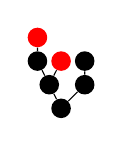
\begin{tikzpicture}[scale=.2]
\node[circle, scale=0.75, fill] (tid0) at (2.25,0){};
\node[circle, scale=0.75, fill] (tid1) at (1.5,1.5){};
\node[circle, scale=0.75, fill] (tid3) at (0.75,3){};
\node[circle, scale=0.75, fill, red] (tid6) at (0.75,4.5){};
\draw[](tid3) -- (tid6);
\node[circle, scale=0.75, fill, red] (tid4) at (2.25,3){};
\draw[](tid1) -- (tid3);
\draw[](tid1) -- (tid4);
\node[circle, scale=0.75, fill] (tid2) at (3.75,1.5){};
\node[circle, scale=0.75, fill] (tid5) at (3.75,3){};
\draw[](tid2) -- (tid5);
\draw[](tid0) -- (tid1);
\draw[](tid0) -- (tid2);

\end{tikzpicture}
\nodepart{two}
\footnotesize{4.84375}
};
\draw (sn0x8df5a88W11.south) -- (sn0x8df2a00W-13.north);
\draw (sn0x8df5a88W11.south) -- (sn0x8df3d10W-2.north);
\draw (sn0x8df5a88W11.south) -- (sn0x8df3ca8W-8.north);
\node[draw=black, rectangle split, rectangle split parts=2] (sn0x8df5bf0W17) at (17.75, -60) {
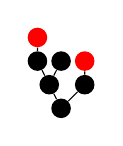
\begin{tikzpicture}[scale=.2]
\node[circle, scale=0.75, fill] (tid0) at (2.25,0){};
\node[circle, scale=0.75, fill] (tid1) at (1.5,1.5){};
\node[circle, scale=0.75, fill] (tid3) at (0.75,3){};
\node[circle, scale=0.75, fill, red] (tid6) at (0.75,4.5){};
\draw[](tid3) -- (tid6);
\node[circle, scale=0.75, fill] (tid4) at (2.25,3){};
\draw[](tid1) -- (tid3);
\draw[](tid1) -- (tid4);
\node[circle, scale=0.75, fill] (tid2) at (3.75,1.5){};
\node[circle, scale=0.75, fill, red] (tid5) at (3.75,3){};
\draw[](tid2) -- (tid5);
\draw[](tid0) -- (tid1);
\draw[](tid0) -- (tid2);

\end{tikzpicture}
\nodepart{two}
\footnotesize{4.84375}
};
\draw (sn0x8df5bf0W17.south) -- (sn0x8df55d8W12.north);
\draw (sn0x8df5bf0W17.south) -- (sn0x8df3ca8W-8.north);
\draw (sn0x8df5128W7.south) -- (sn0x8df5a88W11.north);
\draw (sn0x8df5128W7.south) -- (sn0x8df5bf0W17.north);
\draw (sn0x8df5128W7.south) -- (sn0x8df3ee0W-4.north);
\draw (sn0x8df5128W7.south) -- (sn0x8df44e0W-12.north);
\draw (sn0x8df06c8W-4.south) -- (sn0x8df4bf8W0.north);
\draw (sn0x8df06c8W-4.south) -- (sn0x8df5128W7.north);
\draw (sn0x8df06c8W-4.south) -- (sn0x8df1ec8W-8.north);
\draw (sn0x8df10a8W-13.south) -- (sn0x8df1010W-12.north);
\draw (sn0x8df10a8W-13.south) -- (sn0x8df06c8W-4.north);
\node[draw=black, rectangle split, rectangle split parts=2] (sn0x8df02f8W-5) at (-5.5, -24) {
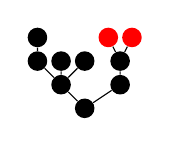
\begin{tikzpicture}[scale=.2]
\node[circle, scale=0.75, fill] (tid0) at (3.75,0){};
\node[circle, scale=0.75, fill] (tid1) at (2.25,1.5){};
\node[circle, scale=0.75, fill] (tid4) at (0.75,3){};
\node[circle, scale=0.75, fill] (tid9) at (0.75,4.5){};
\draw[](tid4) -- (tid9);
\node[circle, scale=0.75, fill] (tid5) at (2.25,3){};
\node[circle, scale=0.75, fill] (tid6) at (3.75,3){};
\draw[](tid1) -- (tid4);
\draw[](tid1) -- (tid5);
\draw[](tid1) -- (tid6);
\node[circle, scale=0.75, fill] (tid2) at (6,1.5){};
\node[circle, scale=0.75, fill] (tid3) at (6,3){};
\node[circle, scale=0.75, fill, red] (tid7) at (5.25,4.5){};
\node[circle, scale=0.75, fill, red] (tid8) at (6.75,4.5){};
\draw[](tid3) -- (tid7);
\draw[](tid3) -- (tid8);
\draw[](tid2) -- (tid3);
\draw[](tid0) -- (tid1);
\draw[](tid0) -- (tid2);

\end{tikzpicture}
\nodepart{two}
\footnotesize{6.29688}
};
\draw (sn0x8df02f8W-5.south) -- (sn0x8df06c8W-4.north);
\node[draw=black, rectangle split, rectangle split parts=2] (sn0x8df0168W4) at (4, -24) {
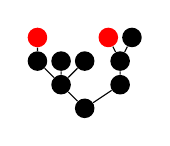
\begin{tikzpicture}[scale=.2]
\node[circle, scale=0.75, fill] (tid0) at (3.75,0){};
\node[circle, scale=0.75, fill] (tid1) at (2.25,1.5){};
\node[circle, scale=0.75, fill] (tid4) at (0.75,3){};
\node[circle, scale=0.75, fill, red] (tid9) at (0.75,4.5){};
\draw[](tid4) -- (tid9);
\node[circle, scale=0.75, fill] (tid5) at (2.25,3){};
\node[circle, scale=0.75, fill] (tid6) at (3.75,3){};
\draw[](tid1) -- (tid4);
\draw[](tid1) -- (tid5);
\draw[](tid1) -- (tid6);
\node[circle, scale=0.75, fill] (tid2) at (6,1.5){};
\node[circle, scale=0.75, fill] (tid3) at (6,3){};
\node[circle, scale=0.75, fill, red] (tid7) at (5.25,4.5){};
\node[circle, scale=0.75, fill] (tid8) at (6.75,4.5){};
\draw[](tid3) -- (tid7);
\draw[](tid3) -- (tid8);
\draw[](tid2) -- (tid3);
\draw[](tid0) -- (tid1);
\draw[](tid0) -- (tid2);

\end{tikzpicture}
\nodepart{two}
\footnotesize{6.29688}
};
\node[draw=black, rectangle split, rectangle split parts=2] (sn0x8df64c8W3) at (3.25, -36) {
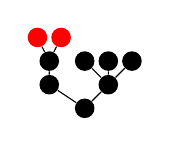
\begin{tikzpicture}[scale=.2]
\node[circle, scale=0.75, fill] (tid0) at (3.75,0){};
\node[circle, scale=0.75, fill] (tid1) at (1.5,1.5){};
\node[circle, scale=0.75, fill] (tid3) at (1.5,3){};
\node[circle, scale=0.75, fill, red] (tid7) at (0.75,4.5){};
\node[circle, scale=0.75, fill, red] (tid8) at (2.25,4.5){};
\draw[](tid3) -- (tid7);
\draw[](tid3) -- (tid8);
\draw[](tid1) -- (tid3);
\node[circle, scale=0.75, fill] (tid2) at (5.25,1.5){};
\node[circle, scale=0.75, fill] (tid4) at (3.75,3){};
\node[circle, scale=0.75, fill] (tid5) at (5.25,3){};
\node[circle, scale=0.75, fill] (tid6) at (6.75,3){};
\draw[](tid2) -- (tid4);
\draw[](tid2) -- (tid5);
\draw[](tid2) -- (tid6);
\draw[](tid0) -- (tid1);
\draw[](tid0) -- (tid2);

\end{tikzpicture}
\nodepart{two}
\footnotesize{5.79688}
};
\draw (sn0x8df64c8W3.south) -- (sn0x8df1ec8W-8.north);
\draw (sn0x8df0168W4.south) -- (sn0x8df06c8W-4.north);
\draw (sn0x8df0168W4.south) -- (sn0x8df64c8W3.north);
\draw (sn0x8def9a0W-4.south) -- (sn0x8df10a8W-13.north);
\draw (sn0x8def9a0W-4.south) -- (sn0x8df02f8W-5.north);
\draw (sn0x8def9a0W-4.south) -- (sn0x8df0168W4.north);
\end{tikzpicture}

%%% Local Variables:
%%% TeX-master: "thesis/thesis.tex"
%%% End: 

\begin{tikzpicture}[scale=.2, anchor=south west]
\node[draw=black, rectangle split, rectangle split parts=2] (sn0x8defa00W-4) at (-4.75, -12) {
\begin{tikzpicture}[scale=.2]
\node[circle, scale=0.75, fill] (tid0) at (3.75,0){};
\node[circle, scale=0.75, fill] (tid1) at (1.5,1.5){};
\node[circle, scale=0.75, fill] (tid3) at (1.5,3){};
\node[circle, scale=0.75, fill] (tid7) at (0.75,4.5){};
\node[circle, scale=0.75, fill, red] (tid10) at (0.75,6){};
\draw[](tid7) -- (tid10);
\node[circle, scale=0.75, fill] (tid8) at (2.25,4.5){};
\draw[](tid3) -- (tid7);
\draw[](tid3) -- (tid8);
\draw[](tid1) -- (tid3);
\node[circle, scale=0.75, fill] (tid2) at (5.25,1.5){};
\node[circle, scale=0.75, fill] (tid4) at (3.75,3){};
\node[circle, scale=0.75, fill, red] (tid9) at (3.75,4.5){};
\draw[](tid4) -- (tid9);
\node[circle, scale=0.75, fill] (tid5) at (5.25,3){};
\node[circle, scale=0.75, fill] (tid6) at (6.75,3){};
\draw[](tid2) -- (tid4);
\draw[](tid2) -- (tid5);
\draw[](tid2) -- (tid6);
\draw[](tid0) -- (tid1);
\draw[](tid0) -- (tid2);

\end{tikzpicture}
\nodepart{two}
\footnotesize{6.82812}
};
\node[draw=black, rectangle split, rectangle split parts=2] (sn0x8df60a0W-9) at (-9.5, -24) {
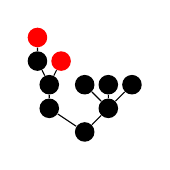
\begin{tikzpicture}[scale=.2]
\node[circle, scale=0.75, fill] (tid0) at (3.75,0){};
\node[circle, scale=0.75, fill] (tid1) at (1.5,1.5){};
\node[circle, scale=0.75, fill] (tid3) at (1.5,3){};
\node[circle, scale=0.75, fill] (tid7) at (0.75,4.5){};
\node[circle, scale=0.75, fill, red] (tid9) at (0.75,6){};
\draw[](tid7) -- (tid9);
\node[circle, scale=0.75, fill, red] (tid8) at (2.25,4.5){};
\draw[](tid3) -- (tid7);
\draw[](tid3) -- (tid8);
\draw[](tid1) -- (tid3);
\node[circle, scale=0.75, fill] (tid2) at (5.25,1.5){};
\node[circle, scale=0.75, fill] (tid4) at (3.75,3){};
\node[circle, scale=0.75, fill] (tid5) at (5.25,3){};
\node[circle, scale=0.75, fill] (tid6) at (6.75,3){};
\draw[](tid2) -- (tid4);
\draw[](tid2) -- (tid5);
\draw[](tid2) -- (tid6);
\draw[](tid0) -- (tid1);
\draw[](tid0) -- (tid2);

\end{tikzpicture}
\nodepart{two}
\footnotesize{6.35938}
};
\node[draw=black, rectangle split, rectangle split parts=2] (sn0x8df1010W-12) at (-12.75, -36) {
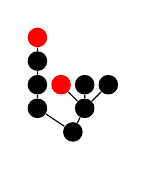
\begin{tikzpicture}[scale=.2]
\node[circle, scale=0.75, fill] (tid0) at (3,0){};
\node[circle, scale=0.75, fill] (tid1) at (0.75,1.5){};
\node[circle, scale=0.75, fill] (tid3) at (0.75,3){};
\node[circle, scale=0.75, fill] (tid7) at (0.75,4.5){};
\node[circle, scale=0.75, fill, red] (tid8) at (0.75,6){};
\draw[](tid7) -- (tid8);
\draw[](tid3) -- (tid7);
\draw[](tid1) -- (tid3);
\node[circle, scale=0.75, fill] (tid2) at (3.75,1.5){};
\node[circle, scale=0.75, fill, red] (tid4) at (2.25,3){};
\node[circle, scale=0.75, fill] (tid5) at (3.75,3){};
\node[circle, scale=0.75, fill] (tid6) at (5.25,3){};
\draw[](tid2) -- (tid4);
\draw[](tid2) -- (tid5);
\draw[](tid2) -- (tid6);
\draw[](tid0) -- (tid1);
\draw[](tid0) -- (tid2);

\end{tikzpicture}
\nodepart{two}
\footnotesize{5.92188}
};
\node[draw=black, rectangle split, rectangle split parts=2] (sn0x8df17c0W-15) at (-15.25, -48) {
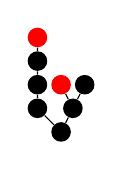
\begin{tikzpicture}[scale=.2]
\node[circle, scale=0.75, fill] (tid0) at (2.25,0){};
\node[circle, scale=0.75, fill] (tid1) at (0.75,1.5){};
\node[circle, scale=0.75, fill] (tid3) at (0.75,3){};
\node[circle, scale=0.75, fill] (tid6) at (0.75,4.5){};
\node[circle, scale=0.75, fill, red] (tid7) at (0.75,6){};
\draw[](tid6) -- (tid7);
\draw[](tid3) -- (tid6);
\draw[](tid1) -- (tid3);
\node[circle, scale=0.75, fill] (tid2) at (3,1.5){};
\node[circle, scale=0.75, fill, red] (tid4) at (2.25,3){};
\node[circle, scale=0.75, fill] (tid5) at (3.75,3){};
\draw[](tid2) -- (tid4);
\draw[](tid2) -- (tid5);
\draw[](tid0) -- (tid1);
\draw[](tid0) -- (tid2);

\end{tikzpicture}
\nodepart{two}
\footnotesize{5.54688}
};
\node[draw=black, rectangle split, rectangle split parts=2] (sn0x8df2260W-24) at (-24.25, -60) {
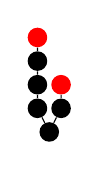
\begin{tikzpicture}[scale=.2]
\node[circle, scale=0.75, fill] (tid0) at (1.5,0){};
\node[circle, scale=0.75, fill] (tid1) at (0.75,1.5){};
\node[circle, scale=0.75, fill] (tid3) at (0.75,3){};
\node[circle, scale=0.75, fill] (tid5) at (0.75,4.5){};
\node[circle, scale=0.75, fill, red] (tid6) at (0.75,6){};
\draw[](tid5) -- (tid6);
\draw[](tid3) -- (tid5);
\draw[](tid1) -- (tid3);
\node[circle, scale=0.75, fill] (tid2) at (2.25,1.5){};
\node[circle, scale=0.75, fill, red] (tid4) at (2.25,3){};
\draw[](tid2) -- (tid4);
\draw[](tid0) -- (tid1);
\draw[](tid0) -- (tid2);

\end{tikzpicture}
\nodepart{two}
\footnotesize{5.25}
};
\node[draw=black, rectangle split, rectangle split parts=2] (sn0x8df2658W-18) at (-18.75, -72) {
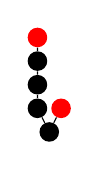
\begin{tikzpicture}[scale=.2]
\node[circle, scale=0.75, fill] (tid0) at (1.5,0){};
\node[circle, scale=0.75, fill] (tid1) at (0.75,1.5){};
\node[circle, scale=0.75, fill] (tid3) at (0.75,3){};
\node[circle, scale=0.75, fill] (tid4) at (0.75,4.5){};
\node[circle, scale=0.75, fill, red] (tid5) at (0.75,6){};
\draw[](tid4) -- (tid5);
\draw[](tid3) -- (tid4);
\draw[](tid1) -- (tid3);
\node[circle, scale=0.75, fill, red] (tid2) at (2.25,1.5){};
\draw[](tid0) -- (tid1);
\draw[](tid0) -- (tid2);

\end{tikzpicture}
\nodepart{two}
\footnotesize{5.0625}
};
\node[draw=black, rectangle split, rectangle split parts=2] (sn0x8df2c20W-10) at (-10, -84) {
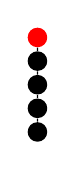
\begin{tikzpicture}[scale=.2]
\node[circle, scale=0.75, fill] (tid0) at (0.75,0){};
\node[circle, scale=0.75, fill] (tid1) at (0.75,1.5){};
\node[circle, scale=0.75, fill] (tid2) at (0.75,3){};
\node[circle, scale=0.75, fill] (tid3) at (0.75,4.5){};
\node[circle, scale=0.75, fill, red] (tid4) at (0.75,6){};
\draw[](tid3) -- (tid4);
\draw[](tid2) -- (tid3);
\draw[](tid1) -- (tid2);
\draw[](tid0) -- (tid1);

\end{tikzpicture}
\nodepart{two}
\footnotesize{5}
};
\node[draw=black, rectangle split, rectangle split parts=2] (sn0x8df2f28W-4) at (-4.25, -96) {
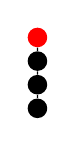
\begin{tikzpicture}[scale=.2]
\node[circle, scale=0.75, fill] (tid0) at (0.75,0){};
\node[circle, scale=0.75, fill] (tid1) at (0.75,1.5){};
\node[circle, scale=0.75, fill] (tid2) at (0.75,3){};
\node[circle, scale=0.75, fill, red] (tid3) at (0.75,4.5){};
\draw[](tid2) -- (tid3);
\draw[](tid1) -- (tid2);
\draw[](tid0) -- (tid1);

\end{tikzpicture}
\nodepart{two}
\footnotesize{4}
};
\node[draw=black, rectangle split, rectangle split parts=2] (sn0x8df2fc0W-4) at (-4.25, -108) {
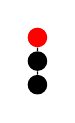
\begin{tikzpicture}[scale=.2]
\node[circle, scale=0.75, fill] (tid0) at (0.75,0){};
\node[circle, scale=0.75, fill] (tid1) at (0.75,1.5){};
\node[circle, scale=0.75, fill, red] (tid2) at (0.75,3){};
\draw[](tid1) -- (tid2);
\draw[](tid0) -- (tid1);

\end{tikzpicture}
\nodepart{two}
\footnotesize{3}
};
\node[draw=black, rectangle split, rectangle split parts=2] (sn0x8df30c0W-1) at (-1.75, -120) {

\begin{tikzpicture}[scale=.2]
\node[circle, scale=0.75, fill] (tid0) at (0.75,0){};
\node[circle, scale=0.75, fill, red] (tid1) at (0.75,1.5){};
\draw[](tid0) -- (tid1);

\end{tikzpicture}
\nodepart{two}
\footnotesize{2}
};
\draw (sn0x8df2fc0W-4.south) -- (sn0x8df30c0W-1.north);
\draw (sn0x8df2f28W-4.south) -- (sn0x8df2fc0W-4.north);
\draw (sn0x8df2c20W-10.south) -- (sn0x8df2f28W-4.north);
\node[draw=black, rectangle split, rectangle split parts=2] (sn0x8df2d88W-6) at (-6.5, -84) {
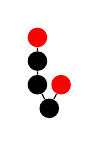
\begin{tikzpicture}[scale=.2]
\node[circle, scale=0.75, fill] (tid0) at (1.5,0){};
\node[circle, scale=0.75, fill] (tid1) at (0.75,1.5){};
\node[circle, scale=0.75, fill] (tid3) at (0.75,3){};
\node[circle, scale=0.75, fill, red] (tid4) at (0.75,4.5){};
\draw[](tid3) -- (tid4);
\draw[](tid1) -- (tid3);
\node[circle, scale=0.75, fill, red] (tid2) at (2.25,1.5){};
\draw[](tid0) -- (tid1);
\draw[](tid0) -- (tid2);

\end{tikzpicture}
\nodepart{two}
\footnotesize{4.125}
};
\node[draw=black, rectangle split, rectangle split parts=2] (sn0x8df3410W0) at (-0.75, -96) {
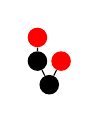
\begin{tikzpicture}[scale=.2]
\node[circle, scale=0.75, fill] (tid0) at (1.5,0){};
\node[circle, scale=0.75, fill] (tid1) at (0.75,1.5){};
\node[circle, scale=0.75, fill, red] (tid3) at (0.75,3){};
\draw[](tid1) -- (tid3);
\node[circle, scale=0.75, fill, red] (tid2) at (2.25,1.5){};
\draw[](tid0) -- (tid1);
\draw[](tid0) -- (tid2);

\end{tikzpicture}
\nodepart{two}
\footnotesize{3.25}
};
\node[draw=black, rectangle split, rectangle split parts=2] (sn0x8df3608W0) at (-0.75, -108) {

\begin{tikzpicture}[scale=.2]
\node[circle, scale=0.75, fill] (tid0) at (1.5,0){};
\node[circle, scale=0.75, fill, red] (tid1) at (0.75,1.5){};
\node[circle, scale=0.75, fill, red] (tid2) at (2.25,1.5){};
\draw[](tid0) -- (tid1);
\draw[](tid0) -- (tid2);

\end{tikzpicture}
\nodepart{two}
\footnotesize{2.5}
};
\draw (sn0x8df3608W0.south) -- (sn0x8df30c0W-1.north);
\draw (sn0x8df3410W0.south) -- (sn0x8df2fc0W-4.north);
\draw (sn0x8df3410W0.south) -- (sn0x8df3608W0.north);
\draw (sn0x8df2d88W-6.south) -- (sn0x8df2f28W-4.north);
\draw (sn0x8df2d88W-6.south) -- (sn0x8df3410W0.north);
\draw (sn0x8df2658W-18.south) -- (sn0x8df2c20W-10.north);
\draw (sn0x8df2658W-18.south) -- (sn0x8df2d88W-6.north);
\node[draw=black, rectangle split, rectangle split parts=2] (sn0x8df2a00W-13) at (-13.75, -72) {
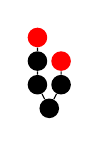
\begin{tikzpicture}[scale=.2]
\node[circle, scale=0.75, fill] (tid0) at (1.5,0){};
\node[circle, scale=0.75, fill] (tid1) at (0.75,1.5){};
\node[circle, scale=0.75, fill] (tid3) at (0.75,3){};
\node[circle, scale=0.75, fill, red] (tid5) at (0.75,4.5){};
\draw[](tid3) -- (tid5);
\draw[](tid1) -- (tid3);
\node[circle, scale=0.75, fill] (tid2) at (2.25,1.5){};
\node[circle, scale=0.75, fill, red] (tid4) at (2.25,3){};
\draw[](tid2) -- (tid4);
\draw[](tid0) -- (tid1);
\draw[](tid0) -- (tid2);

\end{tikzpicture}
\nodepart{two}
\footnotesize{4.4375}
};
\node[draw=black, rectangle split, rectangle split parts=2] (sn0x8df3570W-1) at (-1.5, -84) {
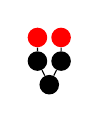
\begin{tikzpicture}[scale=.2]
\node[circle, scale=0.75, fill] (tid0) at (1.5,0){};
\node[circle, scale=0.75, fill] (tid1) at (0.75,1.5){};
\node[circle, scale=0.75, fill, red] (tid3) at (0.75,3){};
\draw[](tid1) -- (tid3);
\node[circle, scale=0.75, fill] (tid2) at (2.25,1.5){};
\node[circle, scale=0.75, fill, red] (tid4) at (2.25,3){};
\draw[](tid2) -- (tid4);
\draw[](tid0) -- (tid1);
\draw[](tid0) -- (tid2);

\end{tikzpicture}
\nodepart{two}
\footnotesize{3.75}
};
\draw (sn0x8df3570W-1.south) -- (sn0x8df3410W0.north);
\draw (sn0x8df2a00W-13.south) -- (sn0x8df2d88W-6.north);
\draw (sn0x8df2a00W-13.south) -- (sn0x8df3570W-1.north);
\draw (sn0x8df2260W-24.south) -- (sn0x8df2658W-18.north);
\draw (sn0x8df2260W-24.south) -- (sn0x8df2a00W-13.north);
\node[draw=black, rectangle split, rectangle split parts=2] (sn0x8df2070W-19) at (-19.25, -60) {
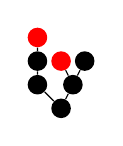
\begin{tikzpicture}[scale=.2]
\node[circle, scale=0.75, fill] (tid0) at (2.25,0){};
\node[circle, scale=0.75, fill] (tid1) at (0.75,1.5){};
\node[circle, scale=0.75, fill] (tid3) at (0.75,3){};
\node[circle, scale=0.75, fill, red] (tid6) at (0.75,4.5){};
\draw[](tid3) -- (tid6);
\draw[](tid1) -- (tid3);
\node[circle, scale=0.75, fill] (tid2) at (3,1.5){};
\node[circle, scale=0.75, fill, red] (tid4) at (2.25,3){};
\node[circle, scale=0.75, fill] (tid5) at (3.75,3){};
\draw[](tid2) -- (tid4);
\draw[](tid2) -- (tid5);
\draw[](tid0) -- (tid1);
\draw[](tid0) -- (tid2);

\end{tikzpicture}
\nodepart{two}
\footnotesize{4.84375}
};
\node[draw=black, rectangle split, rectangle split parts=2] (sn0x8df3ca8W-8) at (-8.75, -72) {
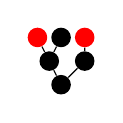
\begin{tikzpicture}[scale=.2]
\node[circle, scale=0.75, fill] (tid0) at (2.25,0){};
\node[circle, scale=0.75, fill] (tid1) at (1.5,1.5){};
\node[circle, scale=0.75, fill, red] (tid3) at (0.75,3){};
\node[circle, scale=0.75, fill] (tid4) at (2.25,3){};
\draw[](tid1) -- (tid3);
\draw[](tid1) -- (tid4);
\node[circle, scale=0.75, fill] (tid2) at (3.75,1.5){};
\node[circle, scale=0.75, fill, red] (tid5) at (3.75,3){};
\draw[](tid2) -- (tid5);
\draw[](tid0) -- (tid1);
\draw[](tid0) -- (tid2);

\end{tikzpicture}
\nodepart{two}
\footnotesize{4.25}
};
\node[draw=black, rectangle split, rectangle split parts=2] (sn0x8df4250W3) at (3.5, -84) {
\begin{tikzpicture}[scale=.2]
\node[circle, scale=0.75, fill] (tid0) at (2.25,0){};
\node[circle, scale=0.75, fill] (tid1) at (1.5,1.5){};
\node[circle, scale=0.75, fill, red] (tid3) at (0.75,3){};
\node[circle, scale=0.75, fill, red] (tid4) at (2.25,3){};
\draw[](tid1) -- (tid3);
\draw[](tid1) -- (tid4);
\node[circle, scale=0.75, fill] (tid2) at (3.75,1.5){};
\draw[](tid0) -- (tid1);
\draw[](tid0) -- (tid2);

\end{tikzpicture}
\nodepart{two}
\footnotesize{3.75}
};
\draw (sn0x8df4250W3.south) -- (sn0x8df3410W0.north);
\draw (sn0x8df3ca8W-8.south) -- (sn0x8df3570W-1.north);
\draw (sn0x8df3ca8W-8.south) -- (sn0x8df4250W3.north);
\node[draw=black, rectangle split, rectangle split parts=2] (sn0x8df3d10W-2) at (-2.25, -72) {
\begin{tikzpicture}[scale=.2]
\node[circle, scale=0.75, fill] (tid0) at (2.25,0){};
\node[circle, scale=0.75, fill] (tid1) at (1.5,1.5){};
\node[circle, scale=0.75, fill, red] (tid3) at (0.75,3){};
\node[circle, scale=0.75, fill, red] (tid4) at (2.25,3){};
\draw[](tid1) -- (tid3);
\draw[](tid1) -- (tid4);
\node[circle, scale=0.75, fill] (tid2) at (3.75,1.5){};
\node[circle, scale=0.75, fill] (tid5) at (3.75,3){};
\draw[](tid2) -- (tid5);
\draw[](tid0) -- (tid1);
\draw[](tid0) -- (tid2);

\end{tikzpicture}
\nodepart{two}
\footnotesize{4.25}
};
\draw (sn0x8df3d10W-2.south) -- (sn0x8df3570W-1.north);
\draw (sn0x8df2070W-19.south) -- (sn0x8df2a00W-13.north);
\draw (sn0x8df2070W-19.south) -- (sn0x8df3ca8W-8.north);
\draw (sn0x8df2070W-19.south) -- (sn0x8df3d10W-2.north);
\draw (sn0x8df17c0W-15.south) -- (sn0x8df2260W-24.north);
\draw (sn0x8df17c0W-15.south) -- (sn0x8df2070W-19.north);
\node[draw=black, rectangle split, rectangle split parts=2] (sn0x8df1ec8W-8) at (-8.75, -48) {
\begin{tikzpicture}[scale=.2]
\node[circle, scale=0.75, fill] (tid0) at (3,0){};
\node[circle, scale=0.75, fill] (tid1) at (2.25,1.5){};
\node[circle, scale=0.75, fill, red] (tid4) at (0.75,3){};
\node[circle, scale=0.75, fill] (tid5) at (2.25,3){};
\node[circle, scale=0.75, fill] (tid6) at (3.75,3){};
\draw[](tid1) -- (tid4);
\draw[](tid1) -- (tid5);
\draw[](tid1) -- (tid6);
\node[circle, scale=0.75, fill] (tid2) at (5.25,1.5){};
\node[circle, scale=0.75, fill] (tid3) at (5.25,3){};
\node[circle, scale=0.75, fill, red] (tid7) at (5.25,4.5){};
\draw[](tid3) -- (tid7);
\draw[](tid2) -- (tid3);
\draw[](tid0) -- (tid1);
\draw[](tid0) -- (tid2);

\end{tikzpicture}
\nodepart{two}
\footnotesize{5.29688}
};
\node[draw=black, rectangle split, rectangle split parts=2] (sn0x8df44e0W-12) at (-12.75, -60) {
\begin{tikzpicture}[scale=.2]
\node[circle, scale=0.75, fill] (tid0) at (3,0){};
\node[circle, scale=0.75, fill] (tid1) at (2.25,1.5){};
\node[circle, scale=0.75, fill, red] (tid3) at (0.75,3){};
\node[circle, scale=0.75, fill] (tid4) at (2.25,3){};
\node[circle, scale=0.75, fill] (tid5) at (3.75,3){};
\draw[](tid1) -- (tid3);
\draw[](tid1) -- (tid4);
\draw[](tid1) -- (tid5);
\node[circle, scale=0.75, fill] (tid2) at (5.25,1.5){};
\node[circle, scale=0.75, fill, red] (tid6) at (5.25,3){};
\draw[](tid2) -- (tid6);
\draw[](tid0) -- (tid1);
\draw[](tid0) -- (tid2);

\end{tikzpicture}
\nodepart{two}
\footnotesize{4.75}
};
\node[draw=black, rectangle split, rectangle split parts=2] (sn0x8df4ab8W4) at (4.25, -72) {
\begin{tikzpicture}[scale=.2]
\node[circle, scale=0.75, fill] (tid0) at (3,0){};
\node[circle, scale=0.75, fill] (tid1) at (2.25,1.5){};
\node[circle, scale=0.75, fill, red] (tid3) at (0.75,3){};
\node[circle, scale=0.75, fill, red] (tid4) at (2.25,3){};
\node[circle, scale=0.75, fill] (tid5) at (3.75,3){};
\draw[](tid1) -- (tid3);
\draw[](tid1) -- (tid4);
\draw[](tid1) -- (tid5);
\node[circle, scale=0.75, fill] (tid2) at (5.25,1.5){};
\draw[](tid0) -- (tid1);
\draw[](tid0) -- (tid2);

\end{tikzpicture}
\nodepart{two}
\footnotesize{4.25}
};
\draw (sn0x8df4ab8W4.south) -- (sn0x8df4250W3.north);
\draw (sn0x8df44e0W-12.south) -- (sn0x8df3ca8W-8.north);
\draw (sn0x8df44e0W-12.south) -- (sn0x8df4ab8W4.north);
\node[draw=black, rectangle split, rectangle split parts=2] (sn0x8df3ee0W-4) at (-4.75, -60) {
\begin{tikzpicture}[scale=.2]
\node[circle, scale=0.75, fill] (tid0) at (3,0){};
\node[circle, scale=0.75, fill] (tid1) at (2.25,1.5){};
\node[circle, scale=0.75, fill, red] (tid3) at (0.75,3){};
\node[circle, scale=0.75, fill, red] (tid4) at (2.25,3){};
\node[circle, scale=0.75, fill] (tid5) at (3.75,3){};
\draw[](tid1) -- (tid3);
\draw[](tid1) -- (tid4);
\draw[](tid1) -- (tid5);
\node[circle, scale=0.75, fill] (tid2) at (5.25,1.5){};
\node[circle, scale=0.75, fill] (tid6) at (5.25,3){};
\draw[](tid2) -- (tid6);
\draw[](tid0) -- (tid1);
\draw[](tid0) -- (tid2);

\end{tikzpicture}
\nodepart{two}
\footnotesize{4.75}
};
\draw (sn0x8df3ee0W-4.south) -- (sn0x8df3d10W-2.north);
\draw (sn0x8df3ee0W-4.south) -- (sn0x8df3ca8W-8.north);
\draw (sn0x8df1ec8W-8.south) -- (sn0x8df2070W-19.north);
\draw (sn0x8df1ec8W-8.south) -- (sn0x8df44e0W-12.north);
\draw (sn0x8df1ec8W-8.south) -- (sn0x8df3ee0W-4.north);
\draw (sn0x8df1010W-12.south) -- (sn0x8df17c0W-15.north);
\draw (sn0x8df1010W-12.south) -- (sn0x8df1ec8W-8.north);
\node[draw=black, rectangle split, rectangle split parts=2] (sn0x8df64c8W-4) at (-4.75, -36) {
\begin{tikzpicture}[scale=.2]
\node[circle, scale=0.75, fill] (tid0) at (3.75,0){};
\node[circle, scale=0.75, fill] (tid1) at (1.5,1.5){};
\node[circle, scale=0.75, fill] (tid3) at (1.5,3){};
\node[circle, scale=0.75, fill, red] (tid7) at (0.75,4.5){};
\node[circle, scale=0.75, fill, red] (tid8) at (2.25,4.5){};
\draw[](tid3) -- (tid7);
\draw[](tid3) -- (tid8);
\draw[](tid1) -- (tid3);
\node[circle, scale=0.75, fill] (tid2) at (5.25,1.5){};
\node[circle, scale=0.75, fill] (tid4) at (3.75,3){};
\node[circle, scale=0.75, fill] (tid5) at (5.25,3){};
\node[circle, scale=0.75, fill] (tid6) at (6.75,3){};
\draw[](tid2) -- (tid4);
\draw[](tid2) -- (tid5);
\draw[](tid2) -- (tid6);
\draw[](tid0) -- (tid1);
\draw[](tid0) -- (tid2);

\end{tikzpicture}
\nodepart{two}
\footnotesize{5.79688}
};
\draw (sn0x8df64c8W-4.south) -- (sn0x8df1ec8W-8.north);
\draw (sn0x8df60a0W-9.south) -- (sn0x8df1010W-12.north);
\draw (sn0x8df60a0W-9.south) -- (sn0x8df64c8W-4.north);
\node[draw=black, rectangle split, rectangle split parts=2] (sn0x8df0168W0) at (0, -24) {
\begin{tikzpicture}[scale=.2]
\node[circle, scale=0.75, fill] (tid0) at (3.75,0){};
\node[circle, scale=0.75, fill] (tid1) at (2.25,1.5){};
\node[circle, scale=0.75, fill] (tid4) at (0.75,3){};
\node[circle, scale=0.75, fill, red] (tid9) at (0.75,4.5){};
\draw[](tid4) -- (tid9);
\node[circle, scale=0.75, fill] (tid5) at (2.25,3){};
\node[circle, scale=0.75, fill] (tid6) at (3.75,3){};
\draw[](tid1) -- (tid4);
\draw[](tid1) -- (tid5);
\draw[](tid1) -- (tid6);
\node[circle, scale=0.75, fill] (tid2) at (6,1.5){};
\node[circle, scale=0.75, fill] (tid3) at (6,3){};
\node[circle, scale=0.75, fill, red] (tid7) at (5.25,4.5){};
\node[circle, scale=0.75, fill] (tid8) at (6.75,4.5){};
\draw[](tid3) -- (tid7);
\draw[](tid3) -- (tid8);
\draw[](tid2) -- (tid3);
\draw[](tid0) -- (tid1);
\draw[](tid0) -- (tid2);

\end{tikzpicture}
\nodepart{two}
\footnotesize{6.29688}
};
\node[draw=black, rectangle split, rectangle split parts=2] (sn0x8df06c8W4) at (4.75, -36) {
\begin{tikzpicture}[scale=.2]
\node[circle, scale=0.75, fill] (tid0) at (3,0){};
\node[circle, scale=0.75, fill] (tid1) at (2.25,1.5){};
\node[circle, scale=0.75, fill] (tid3) at (0.75,3){};
\node[circle, scale=0.75, fill, red] (tid8) at (0.75,4.5){};
\draw[](tid3) -- (tid8);
\node[circle, scale=0.75, fill] (tid5) at (2.25,3){};
\node[circle, scale=0.75, fill] (tid6) at (3.75,3){};
\draw[](tid1) -- (tid3);
\draw[](tid1) -- (tid5);
\draw[](tid1) -- (tid6);
\node[circle, scale=0.75, fill] (tid2) at (5.25,1.5){};
\node[circle, scale=0.75, fill] (tid4) at (5.25,3){};
\node[circle, scale=0.75, fill, red] (tid7) at (5.25,4.5){};
\draw[](tid4) -- (tid7);
\draw[](tid2) -- (tid4);
\draw[](tid0) -- (tid1);
\draw[](tid0) -- (tid2);

\end{tikzpicture}
\nodepart{two}
\footnotesize{5.79688}
};
\node[draw=black, rectangle split, rectangle split parts=2] (sn0x8df4bf8W0) at (-0.75, -48) {
\begin{tikzpicture}[scale=.2]
\node[circle, scale=0.75, fill] (tid0) at (3,0){};
\node[circle, scale=0.75, fill] (tid1) at (2.25,1.5){};
\node[circle, scale=0.75, fill] (tid3) at (0.75,3){};
\node[circle, scale=0.75, fill, red] (tid7) at (0.75,4.5){};
\draw[](tid3) -- (tid7);
\node[circle, scale=0.75, fill] (tid4) at (2.25,3){};
\node[circle, scale=0.75, fill] (tid5) at (3.75,3){};
\draw[](tid1) -- (tid3);
\draw[](tid1) -- (tid4);
\draw[](tid1) -- (tid5);
\node[circle, scale=0.75, fill] (tid2) at (5.25,1.5){};
\node[circle, scale=0.75, fill, red] (tid6) at (5.25,3){};
\draw[](tid2) -- (tid6);
\draw[](tid0) -- (tid1);
\draw[](tid0) -- (tid2);

\end{tikzpicture}
\nodepart{two}
\footnotesize{5.29688}
};
\node[draw=black, rectangle split, rectangle split parts=2] (sn0x8df4dd0W3) at (3.25, -60) {
\begin{tikzpicture}[scale=.2]
\node[circle, scale=0.75, fill] (tid0) at (3,0){};
\node[circle, scale=0.75, fill] (tid1) at (2.25,1.5){};
\node[circle, scale=0.75, fill] (tid3) at (0.75,3){};
\node[circle, scale=0.75, fill, red] (tid6) at (0.75,4.5){};
\draw[](tid3) -- (tid6);
\node[circle, scale=0.75, fill, red] (tid4) at (2.25,3){};
\node[circle, scale=0.75, fill] (tid5) at (3.75,3){};
\draw[](tid1) -- (tid3);
\draw[](tid1) -- (tid4);
\draw[](tid1) -- (tid5);
\node[circle, scale=0.75, fill] (tid2) at (5.25,1.5){};
\draw[](tid0) -- (tid1);
\draw[](tid0) -- (tid2);

\end{tikzpicture}
\nodepart{two}
\footnotesize{4.84375}
};
\node[draw=black, rectangle split, rectangle split parts=2] (sn0x8df55d8W12) at (12.25, -72) {
\begin{tikzpicture}[scale=.2]
\node[circle, scale=0.75, fill] (tid0) at (2.25,0){};
\node[circle, scale=0.75, fill] (tid1) at (1.5,1.5){};
\node[circle, scale=0.75, fill] (tid3) at (0.75,3){};
\node[circle, scale=0.75, fill, red] (tid5) at (0.75,4.5){};
\draw[](tid3) -- (tid5);
\node[circle, scale=0.75, fill, red] (tid4) at (2.25,3){};
\draw[](tid1) -- (tid3);
\draw[](tid1) -- (tid4);
\node[circle, scale=0.75, fill] (tid2) at (3.75,1.5){};
\draw[](tid0) -- (tid1);
\draw[](tid0) -- (tid2);

\end{tikzpicture}
\nodepart{two}
\footnotesize{4.4375}
};
\draw (sn0x8df55d8W12.south) -- (sn0x8df2d88W-6.north);
\draw (sn0x8df55d8W12.south) -- (sn0x8df4250W3.north);
\draw (sn0x8df4dd0W3.south) -- (sn0x8df55d8W12.north);
\draw (sn0x8df4dd0W3.south) -- (sn0x8df4ab8W4.north);
\draw (sn0x8df4bf8W0.south) -- (sn0x8df4dd0W3.north);
\draw (sn0x8df4bf8W0.south) -- (sn0x8df44e0W-12.north);
\node[draw=black, rectangle split, rectangle split parts=2] (sn0x8df5128W7) at (7.25, -48) {
\begin{tikzpicture}[scale=.2]
\node[circle, scale=0.75, fill] (tid0) at (3,0){};
\node[circle, scale=0.75, fill] (tid1) at (2.25,1.5){};
\node[circle, scale=0.75, fill] (tid3) at (0.75,3){};
\node[circle, scale=0.75, fill, red] (tid7) at (0.75,4.5){};
\draw[](tid3) -- (tid7);
\node[circle, scale=0.75, fill, red] (tid4) at (2.25,3){};
\node[circle, scale=0.75, fill] (tid5) at (3.75,3){};
\draw[](tid1) -- (tid3);
\draw[](tid1) -- (tid4);
\draw[](tid1) -- (tid5);
\node[circle, scale=0.75, fill] (tid2) at (5.25,1.5){};
\node[circle, scale=0.75, fill] (tid6) at (5.25,3){};
\draw[](tid2) -- (tid6);
\draw[](tid0) -- (tid1);
\draw[](tid0) -- (tid2);

\end{tikzpicture}
\nodepart{two}
\footnotesize{5.29688}
};
\node[draw=black, rectangle split, rectangle split parts=2] (sn0x8df5a88W11) at (11.25, -60) {
\begin{tikzpicture}[scale=.2]
\node[circle, scale=0.75, fill] (tid0) at (2.25,0){};
\node[circle, scale=0.75, fill] (tid1) at (1.5,1.5){};
\node[circle, scale=0.75, fill] (tid3) at (0.75,3){};
\node[circle, scale=0.75, fill, red] (tid6) at (0.75,4.5){};
\draw[](tid3) -- (tid6);
\node[circle, scale=0.75, fill, red] (tid4) at (2.25,3){};
\draw[](tid1) -- (tid3);
\draw[](tid1) -- (tid4);
\node[circle, scale=0.75, fill] (tid2) at (3.75,1.5){};
\node[circle, scale=0.75, fill] (tid5) at (3.75,3){};
\draw[](tid2) -- (tid5);
\draw[](tid0) -- (tid1);
\draw[](tid0) -- (tid2);

\end{tikzpicture}
\nodepart{two}
\footnotesize{4.84375}
};
\draw (sn0x8df5a88W11.south) -- (sn0x8df2a00W-13.north);
\draw (sn0x8df5a88W11.south) -- (sn0x8df3d10W-2.north);
\draw (sn0x8df5a88W11.south) -- (sn0x8df3ca8W-8.north);
\node[draw=black, rectangle split, rectangle split parts=2] (sn0x8df5bf0W17) at (17.75, -60) {
\begin{tikzpicture}[scale=.2]
\node[circle, scale=0.75, fill] (tid0) at (2.25,0){};
\node[circle, scale=0.75, fill] (tid1) at (1.5,1.5){};
\node[circle, scale=0.75, fill] (tid3) at (0.75,3){};
\node[circle, scale=0.75, fill, red] (tid6) at (0.75,4.5){};
\draw[](tid3) -- (tid6);
\node[circle, scale=0.75, fill] (tid4) at (2.25,3){};
\draw[](tid1) -- (tid3);
\draw[](tid1) -- (tid4);
\node[circle, scale=0.75, fill] (tid2) at (3.75,1.5){};
\node[circle, scale=0.75, fill, red] (tid5) at (3.75,3){};
\draw[](tid2) -- (tid5);
\draw[](tid0) -- (tid1);
\draw[](tid0) -- (tid2);

\end{tikzpicture}
\nodepart{two}
\footnotesize{4.84375}
};
\draw (sn0x8df5bf0W17.south) -- (sn0x8df55d8W12.north);
\draw (sn0x8df5bf0W17.south) -- (sn0x8df3ca8W-8.north);
\draw (sn0x8df5128W7.south) -- (sn0x8df5a88W11.north);
\draw (sn0x8df5128W7.south) -- (sn0x8df5bf0W17.north);
\draw (sn0x8df5128W7.south) -- (sn0x8df3ee0W-4.north);
\draw (sn0x8df5128W7.south) -- (sn0x8df44e0W-12.north);
\draw (sn0x8df06c8W4.south) -- (sn0x8df4bf8W0.north);
\draw (sn0x8df06c8W4.south) -- (sn0x8df5128W7.north);
\draw (sn0x8df06c8W4.south) -- (sn0x8df1ec8W-8.north);
\draw (sn0x8df0168W0.south) -- (sn0x8df06c8W4.north);
\draw (sn0x8df0168W0.south) -- (sn0x8df64c8W-4.north);
\draw (sn0x8defa00W-4.south) -- (sn0x8df60a0W-9.north);
\draw (sn0x8defa00W-4.south) -- (sn0x8df0168W0.north);
\end{tikzpicture}

%%% Local Variables:
%%% TeX-master: "thesis/thesis.tex"
%%% End: 

